\documentclass[11pt,a4paper]{amsart}
\usepackage[utf8]{inputenc}
\usepackage[T1]{fontenc}
\usepackage[colorlinks=true,citecolor=blue,linkcolor=black]{hyperref}
\usepackage{amsmath,mathtools,amssymb,extarrows,mathrsfs,amsthm}
\usepackage{tikz-cd}
\usepackage{tikz}
\usetikzlibrary{backgrounds}
\usetikzlibrary{calc}
\usetikzlibrary{hobby}
\usetikzlibrary{decorations.markings}
\usetikzlibrary{arrows.meta}
\usepackage{xcolor}

\begin{document}

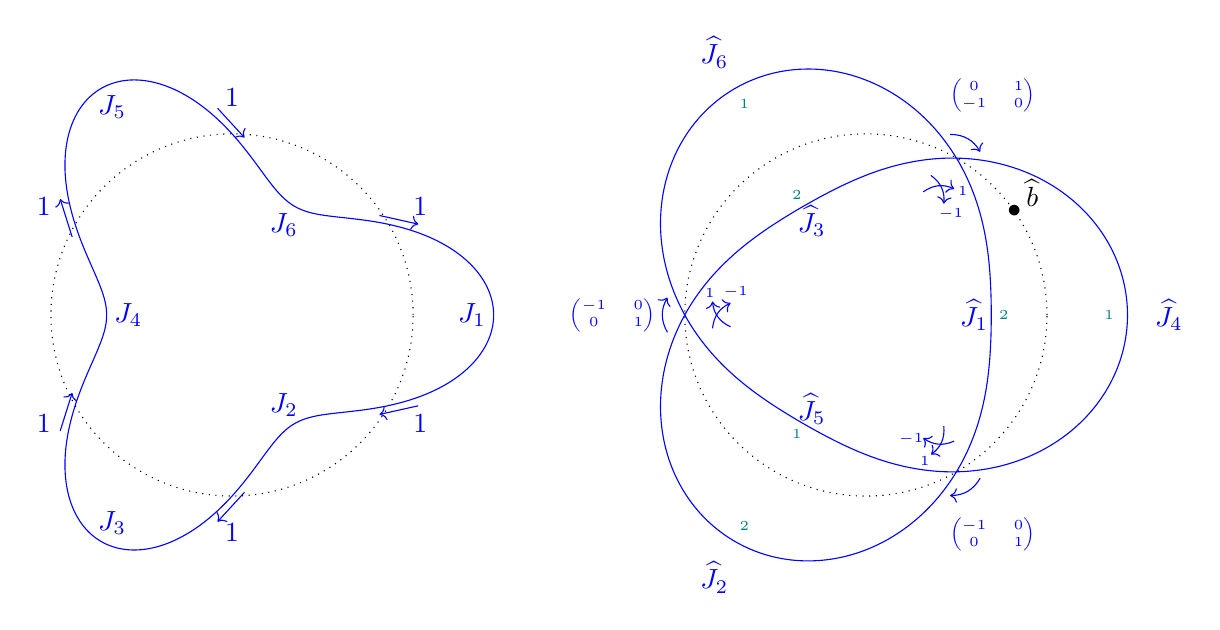
\begin{tikzpicture}[scale=2.3]
	\begin{scope}
		\draw[dotted] (0,0) circle (1);
		\draw[blue,domain=0:(360),scale=1,samples=1000] plot (\x:{exp(-cos(3*\x+180)/exp(1))});  
		\foreach \n in {1,2,...,6} \draw[blue] ({120-(\n+1)*60}:{exp(-cos(3*(120-(\n+1)*60)+180)/exp(1))-0.12}) node {$J_\n$};
		\foreach \n in {1,2,...,6} 
		{\draw[->,blue] ({90-\n*60+4}:{1.06*exp(cos(3*(90-(\n+1)*60+4)+180)/exp(1))}) to ({90-\n*60-4}:{1.06*exp(cos(3*(90-(\n+1)*60-4)+180)/exp(1))});
			\draw[blue] ({90-\n*60}:1.2) node {$1$};
		} 
	\end{scope}
	
	\begin{scope}[xshift=3.5cm]
		\draw[dotted] (0,0) circle (1);
		\draw[blue,domain=0:(2*360),scale=1,samples=1000] plot (\x:{exp(cos(3/2*\x)/exp(1))});  
		\foreach \n in {1,2,...,6} \draw[blue] ({420-\n*120+60}:{exp(1.4*cos(3/2*(420-\n*120)+90)/exp(1))}) node {$\widehat J_\n$};  
		\foreach \n in {0,1,2}
		{\draw[blue,->] ({\n*120+60+5}:0.75) to[bend left] ({\n*120+60-5}:0.85);
			\draw[blue,->] ({\n*120+60+5}:0.85) to[bend left] ({\n*120+60-5}:0.75);
			\draw[blue] ({\n*120+60-8}:0.87) node {{\tiny{$1$}}};
			\draw[blue] ({\n*120+60-10}:0.73) node {{\tiny{$-1$}}};
		}
		\draw[blue,->] ({60+5}:1.1) to[bend left] ({60-5}:1.1);
		\draw[blue] ({60+0}:1.4) node {{\tiny $\begin{pmatrix} 0 & 1 \\ -1 & 0\end{pmatrix}$}};
		\draw[blue,->] ({120+60+5}:1.1) to[bend left] ({120+60-5}:1.1);
		\draw[blue] ({120+60}:1.4) node {{\tiny $\begin{pmatrix} -1 & 0 \\ 0 & 1\end{pmatrix}$}};
		\draw[blue,->] ({-120+60+5}:1.1) to[bend left] ({-120+60-5}:1.1);
		\draw[blue] ({-120+60}:1.4) node {{\tiny $\begin{pmatrix} -1 & 0 \\ 0 & 1\end{pmatrix}$}};
		
		\draw({cos(35)},{sin(35)}) node {$\bullet$};
		\draw({cos(35)+0.1},{sin(35)+0.1}) node {$\widehat{b}$}; 
		\draw[teal] (0:{1.1*exp(-1/exp(1))}) node {\tiny{$2$}};
		\draw[teal] (0:{0.93*exp(1/exp(1))}) node {\tiny{$1$}};
		\draw[teal] (-120:{1.1*exp(-1/exp(1))}) node {\tiny{$1$}};
		\draw[teal] (-120:{0.93*exp(1/exp(1))}) node {\tiny{$2$}};
		\draw[teal] (120:{1.1*exp(-1/exp(1))}) node {\tiny{$2$}};
		\draw[teal] (120:{0.93*exp(1/exp(1))}) node {\tiny{$1$}};
	\end{scope}
\end{tikzpicture}

\end{document}